\documentclass{beamer}
\usepackage{xeCJK}
\usepackage{graphicx}
\usepackage{xcolor}

% ============= setup =============
\usetheme{Madrid}
\usecolortheme{crane}
\setCJKmainfont{Taipei Sans TC Beta}
\setCJKsansfont{Taipei Sans TC Beta}
\setmainfont{Taipei Sans TC Beta}
\hypersetup{
    colorlinks=true,
    linkcolor=black,
    urlcolor=blue
}
\setbeamertemplate{items}[circle]
\setbeamertemplate{section in toc}{\inserttocsectionnumber.~\inserttocsection}
\AtBeginSection[]{
    \begin{frame}
    \vfill
    \centering
    \begin{beamercolorbox}[sep=8pt,center,shadow=true,rounded=true]{title}
        \usebeamerfont{title}\insertsectionhead\par%
    \end{beamercolorbox}
    \vfill
    \end{frame}
}

\title{基礎競賽概論}
\author{temmie}
\date{}
% ============= setup =============

\begin{document}

\begin{frame}
    \titlepage
\end{frame}

\begin{frame}
    \tableofcontents
\end{frame}

\section{賽制介紹}

\begin{frame}
    \frametitle{OI}
    \begin{itemize}
        \item 高中比賽常出現的賽制
        \item 有部份分(子任務)
        \item 子任務用來引導參賽者
    \end{itemize}
\end{frame}

\begin{frame}
    \frametitle{ICPC}
    \begin{itemize}
        \item 大學比賽常出現的賽制
        \item 沒有部份分,比團隊的 AC 數量
        \item<2-> 同 AC 數量則以罰時計算
        \item<2-> 罰時的計算與解題時間和 WA 數量有關
    \end{itemize}
\end{frame}

\begin{frame}
    \frametitle{各種比賽}
    \begin{itemize}
        \item APCS(每年三次)
        \item YTP(7 \~{} 8月)
        \item 學科能力競賽(9 \~{} 12月)
        \item NPSC(11 \~{} 12月)
    \end{itemize}
\end{frame}

\section{複雜度分析}

\begin{frame}
    \frametitle{複雜度的意義}
    \begin{itemize}
        \item 用來客觀衡量一個演算法的標準,包括時間和空間
        \item 通常用資料的數量當作參數,以函數形式呈現
        \item 考慮最差的情況
    \end{itemize}
\end{frame}

\begin{frame}
    \frametitle{為什麼我們需要了解複雜度}
    \begin{itemize}
        \item 可以快速判斷你的程式會不會卡到 TLE、MLE
        \item 比較不同演算法優劣
        \item 可以透過資料數量猜測預期解法
    \end{itemize}
\end{frame}

\begin{frame}
    \frametitle{時間複雜度的例子}
    \begin{block}{圖書館}
        身後有很多書架,你可以用多快的速度找到書?
    \end{block}
    \begin{itemize}
        \item<2-> 我想大部分的人可能是從左到右,從上到下找
        \item<2-> 如果有 $n$ 本書,則你最差需要找 $n$ 次
        \item<3-> 你知道嗎,在某些特殊的情況下,可以在大概 $\log_2{n}$ 次甚至是一次就找到!
    \end{itemize}
\end{frame}

\begin{frame}
    \frametitle{複雜度的表示法}
    \begin{itemize}
        \item 通常會用 $O(...)$ 來表示
        \item 上面的符號叫做 Big-O,用來表示量級的一種趨近上界
        \item<2-> 通常裡面只會丟一種指數量級的參數,例如: $O(n)$、$O(n^2)$
        \item<2-> 如果有較低量級的參數、係數則省略,例如: $O(3n^2+2n+17)$,則表示成 $O(n^2)$
        % 記得用數字代進去舉例
    \end{itemize}
\end{frame}

\begin{frame}
    \frametitle{時間複雜度中的常數}
    \begin{itemize}
        \item 只要是固定操作數量的指令都會計成 $O(1)$
        \item 5次?10次?10000次?
        \item<2-> 這種東西我們稱作\textbf{常數}
        \item<2-> 請注意,即使在時間複雜度上被省略,仍然很重要
        % 可以用 + - * / % 做舉例
    \end{itemize}
\end{frame}

\begin{frame}
    \frametitle{複雜度的量級差異}
    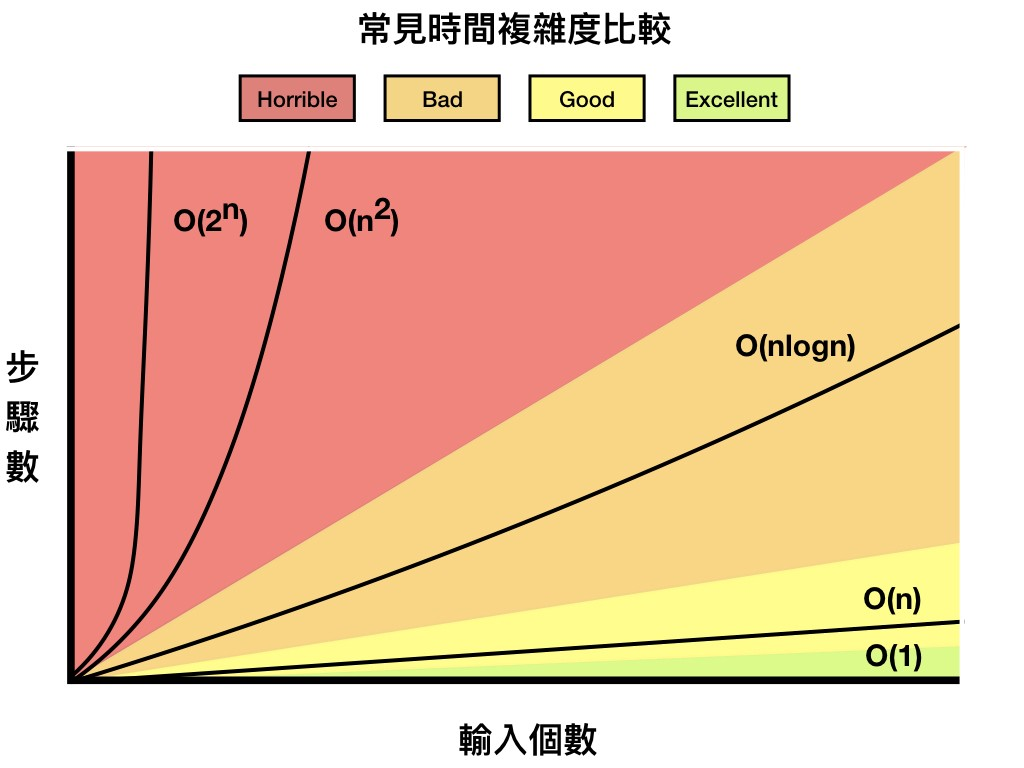
\includegraphics[width=10.0cm]{img/time.png}
\end{frame}

\begin{frame}
    \frametitle{複雜度的量級差異}
    以下為參考的時間複雜度對照量級,估算為約 $10^8$ 操作為一秒
    \begin{itemize}
        \item $O(2^n)$:$n \approx 25$
        \item $O(n^2)$:$n \approx 10^4$
        \item $O(n \log{n})$:$n \approx 5 \times 10^5$
        \item $O(n)$:$n \approx 10^8$
        \item $O(\log{n})$:$n \approx 10^{18}$
        \vspace{0.5cm}
        \item<2-> 背不起來?經驗多就知道了!
    \end{itemize}
\end{frame}

\begin{frame}
    \frametitle{判斷時間複雜度}
    判斷時間複雜度的方法
    \vspace{0.5cm}
    \begin{itemize}
        \item 計算 for 迴圈的層數
        \item 用規律去找
        \item 透過經驗 / 背公式
    \end{itemize}
\end{frame}

\begin{frame}
    \frametitle{例題}
    \begin{block}{複雜度分析練習-1}
        請試著分析下面程式碼的時間複雜度

        \vspace{0.5cm}
        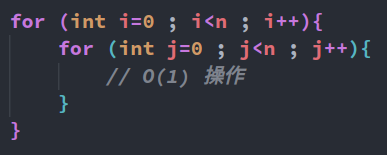
\includegraphics[width=7.0cm]{img/code_1.png}
    \end{block}
    \begin{itemize}
        \item<2-> 我們可以發先第一個 for 迴圈重複 n 次,並且第二個也重複 n 次
        \item<2-> 答案為 $O(n^2)$
    \end{itemize}
\end{frame}

\begin{frame}
    \frametitle{例題}
    \begin{block}{複雜度分析練習-2}
        請試著分析下面程式碼的時間複雜度

        \vspace{0.5cm}
        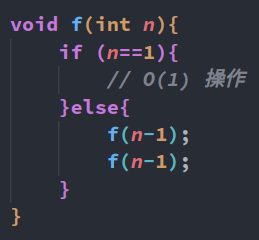
\includegraphics[width=4.0cm]{img/code_2.png}
    
        \begin{itemize}
            \item<2-> 每次遞迴都會增加兩倍的數字,實際上會有 $2^{n-1}$ 次操作
            \item<2-> 答案為 $O(2^n)$
        \end{itemize}
    \end{block}
\end{frame}

\begin{frame}
    \frametitle{作業}
    \begin{itemize}
        \item 回家把這些影片看完,練習看看裡面的題目吧 :D
        \item \href{https://youtube.com/playlist?list=PLuV4P3EY8fXl-2qmLTZVWS3deHyxxWLUI}{AA競程 Level 1 公開課 7\~13}
    \end{itemize}
\end{frame}

\section{雜項}

\begin{frame}
    \frametitle{競程常見數學符號}
    \begin{itemize}
        \item $\displaystyle\sum_{i=1}^{n} i$:連加符號
        \item $\displaystyle\prod_{i=1}^{n} i$:連乘符號
        \vspace{0.5cm}
        \item<2-> $\lceil n \rceil$:無條件進位
        \item<2-> $\lfloor n \rfloor$:無條件捨去
    \end{itemize}
\end{frame}

\begin{frame}
    \frametitle{競程常見數學符號}
    \begin{itemize}
        \item $a \bmod b$:$a \div b$ 的餘數
        \item $a \equiv b \pmod{m}$:$a \bmod m = b \bmod m$
        \item $a \mid b$:a 整除 b
    \end{itemize}
\end{frame}

\begin{frame}
    \frametitle{萬用標頭檔}
    \begin{itemize}
        \item 只要在使用 \#include<bits/stdc++.h> 就可以引入 95\% 會用到的標頭檔
    \end{itemize}
\end{frame}

\begin{frame}
    \frametitle{全域變數}
    \begin{itemize}
        \item 不想學指標?把所有東西都丟進全域吧
        \item 可以開更大的陣列
        \item 可以自動初始化
        \item (還是要學會指標啦)
    \end{itemize}
\end{frame}

\begin{frame}
    \frametitle{IO 加速}
    \begin{itemize}
        \item \href{https://codeforces.com/group/S6XjkGb6qB/contest/403070/problem/A}{先試試看這題吧}
        \item<2-> 如此簡單的題目怎麼過不了?
        \item<3-> 這是因為輸入、輸出太多導致超時
        \item<3-> 可以透過加上 cin.tie(0)、ios::sync\_with\_stdio(0) 和不使用 endl 改用 '$\backslash$ n' 加速
        \item<4-> 想了解原因?私訊我吧
    \end{itemize}
\end{frame}

\begin{frame}
    \frametitle{\#define}
    \begin{itemize}
        \item 總是因為沒開 long long 而 WA 感到很煩躁?
        \item<2-> 我們可以用 \#define 這個函式把所有 int 定義成 long long
        \item<3-> 請記得將原先的 main 改成 signed main(void),否則無法使用
    \end{itemize}
\end{frame}

\begin{frame}
    \frametitle{函式改值}
    \begin{itemize}
        \item 丟進函式裡面的值沒有辦法被更改,但又不想用很毒的全域變數?
        \item 你可以在宣告變數的時候加上 \&,這樣就可以在函式裡面改值囉
        \vspace{0.5cm}
        \item 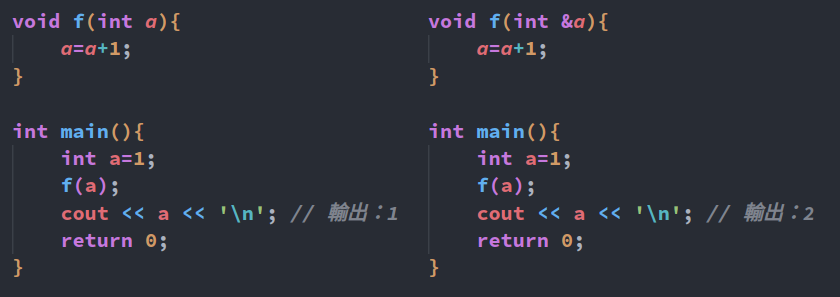
\includegraphics[width=10.0cm]{img/code_3.png}
    \end{itemize}
\end{frame}


\end{document}